\documentclass[tikz,border=4pt]{standalone}
\usepackage[T1]{fontenc}
\usepackage{lmodern}
\usepackage{xcolor}
\definecolor{NordBody}{HTML}{4C566A}
\definecolor{NordBlue}{HTML}{5E81AC}
\definecolor{NordPanel}{HTML}{ECEFF4}
\begin{document}
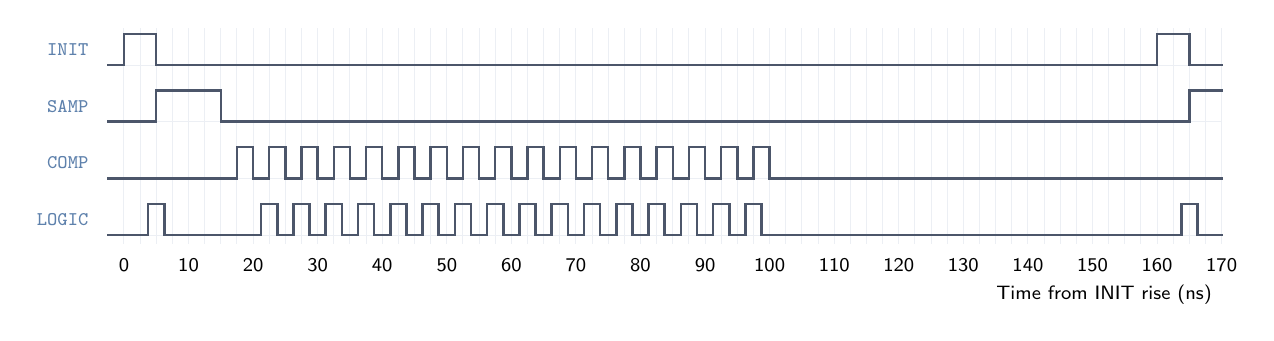
\begin{tikzpicture}[
  x=0.082cm,y=0.72cm,font=\sffamily\scriptsize,
  waveform/.style={draw=NordBody,line width=0.9pt,line join=miter,line cap=rect},
  guide/.style={draw=NordPanel,line width=0.35pt}]
  % Original fixed_input_timing_params recipe at 1.6 Gsymbol/s, relative to INIT.
  % Patterns repeat every 160 ns; LOGIC phase is delayed by two symbols.
  \foreach \t in {0,2.5,...,170} {\draw[guide] (\t,-0.15) -- (\t,3.65);}
  \foreach \y/\name in {3/INIT,2/SAMP,1/COMP,0/LOGIC} {
    \draw[guide] (-2.5,\y) -- (170,\y);
    \node[anchor=east,text=NordBlue,font=\ttfamily\bfseries\scriptsize]
      at (-4,\y+0.275) {\name};
  }
  \draw[waveform] (-2.5,3) -- (0,3) -- (0,3.55) -- (5,3.55) -- (5,3)
    -- (160,3) -- (160,3.55) -- (165,3.55) -- (165,3) -- (170,3);
  \draw[waveform] (-2.5,2) -- (5,2) -- (5,2.55) -- (15,2.55) -- (15,2)
    -- (165,2) -- (165,2.55) -- (170,2.55);
  \draw[waveform] (-2.5,1) -- (17.5,1);
  \foreach \k in {0,...,16} {
    \pgfmathsetmacro{\start}{17.5+5*\k}
    \pgfmathsetmacro{\stop}{\start+2.5}
    \pgfmathsetmacro{\next}{\start+5}
    \draw[waveform] (\start,1) -- (\start,1.55) -- (\stop,1.55)
      -- (\stop,1) -- (\next,1);
  }
  \draw[waveform] (102.5,1) -- (170,1);
  \draw[waveform] (-2.5,0) -- (3.75,0) -- (3.75,0.55) -- (6.25,0.55)
    -- (6.25,0) -- (21.25,0);
  \foreach \k in {0,...,15} {
    \pgfmathsetmacro{\start}{21.25+5*\k}
    \pgfmathsetmacro{\stop}{\start+2.5}
    \pgfmathsetmacro{\next}{\start+5}
    \draw[waveform] (\start,0) -- (\start,0.55) -- (\stop,0.55)
      -- (\stop,0) -- (\next,0);
  }
  \draw[waveform] (101.25,0) -- (163.75,0) -- (163.75,0.55)
    -- (166.25,0.55) -- (166.25,0) -- (170,0);
  \foreach \t in {0,10,...,170} {\node[anchor=north] at (\t,-0.25) {\t};}
  \node[anchor=north east] at (170,-0.7) {Time from INIT rise (ns)};
\end{tikzpicture}
\end{document}
